\chapter{پیاده‌سازی سیستم}

در این قسمت نحوه‌ی اجرای پروژه را بطور کامل توضیح خواهیم داد. در هر قسمت ساختار فایل‌ها، نحوه‌ی پیاده‌سازی و چالش‌هایی که با آن مواجه بودیم به‌همراه نحوه‌ی حل آنها را توضیح خواهیم داد.

\section{معماری کلی سیستم}

برای درک بهتر این پروژه، نمایی کلی از سیستم و نحوه عملکرد آن را همانطور که در \cref{fig:system_overview} نشان داده شده است، ارائه خواهیم داد. این پروژه در چندین محل صنعتی مستقر خواهد شد. در هر کارخانه چندین میکروکنترلر آردوینو، با یک سنسور لرزش و یک فرستنده گیرنده زیگبی متصل، روی هر قطعه از تجهیزات نصب شده است. داده‌ها در زمان‌های برنامه‌ریزی‌شده حس می‌شوند و سپس به دروازه‌ای در کارخانه ارسال می‌شوند. دروازه اطلاعاتی را که از فرستنده‌گیرنده‌های زیگبی می‌آید را جمع‌آوری می‌کند تا زمانی که به یک آستانه‌ی از پیش تعریف‌شده برسد. سپس دروازه با سرور مرکزی احراز هویت می‌شود و سپس داده‌های جمع‌آوری‌شده را با پروتکل \lr{HTTP} به سرور ارسال می‌کند. در سرور مراحل پیش‌پردازش لازم انجام می‌شود و سپس داده‌ها در پایگاه داده‌ی سری زمانی ذخیره می‌شوند. سپس مدل یادگیری ماشین با داده‌های قبلی و جدید اجرا می‌شود تا پیش‌بینی دقیق‌تری درباره طول عمر مفید باقیمانده تجهیزات به ما ارائه دهد. در صورت درخواست، تمام داده‌های تحلیلی و پیشبینی‌ها از طریق داشبورد مدیریت قابل‌دسترسی است. متخصصان می‌توانند از این داده‌ها برای برنامه‌ریزی زمان نگهداری مناسب استفاده کنند.

\begin{figure}[!h]
\centering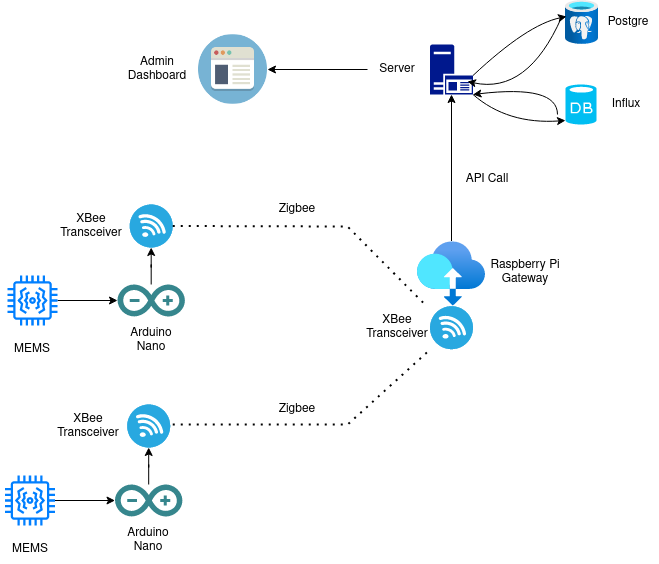
\includegraphics[scale=.6]{system_overview.png}
\caption{نمای کلی سیستم}\label{fig:system_overview}
\end{figure}

\section{گره انتهایی و آردوینو}

برای پیاده‌سازی گره انتهایی، سه بخش را باید پیاده‌سازی میکردیم که عبارتند از:

\begin{itemize}
\item خواندن از حسگر و نمونه‌برداری
\item تشکیل فریم زیگبی و نوشتن در درگاه سریال
\item خوابیدن و بیدارشدن در بازه‌های زمانی مشخص
\end{itemize}

در ادامه هر بخش را توضیح می‌دهیم.

\subsection{خواندن از حسگر و نمونه‌برداری}

حسگر \lr{ADXL345} چندین پارامتر دارد که باید در زمان راه‌اندازی تنظیم شوند. برای انجام پیکربندی و همچنین خواندن داده‌های حسگرها بدون نیاز به استفاده مستقیم از پروتکل \lr{I2C}، از کتابخانه\LTRfootnote{Adafruit\_ADXL345\_U.h} استفاده کرده‌ایم. یکی از پارامترها محدوده شتاب است که با تابع \lr{setRange} تنظیم می‌شود. محدوده مجاز ۲، ۴، ۸ یا ۱۶ برابر شتاب گرانش زمین است. اما هرچه دامنه بزرگتر شود، داده‌ها دقت کمتری پیدا می‌کنند. از آنجایی که یک قطعه از تجهیزات حتی زمانی که قدیمی باشد با شتاب بالا نمی‌لرزد و برای پیش‌بینی‌های دقیق‌تر به دقت نیاز است، تصمیم گرفتیم که محدوده را روی دو برابر شتاب گرانش زمین تنظیم کنیم.


پارامتر دیگر نرخ داده است که باید در زمان راه‌اندازی با استفاده از تابع \lr{setDataRate} تنظیم شود. نرخ داده برای تنظیم نرخ ارتباط بین حسگر و بورد آردوینو از طریق پروتکل \lr{I2C} استفاده می‌شود. بنابراین مهم است که نرخ داده با رسانه‌ی ارتباطی سازگار باشد. از آنجایی که اگر نرخ داده بالاتر از نرخی باشد که رسانه قادر به انجام آن است، برخی از داده‌ها از بین می‌روند. بدلیل برخی چالش‌های دیگر که در ادامه در مورد آنها صحبت خواهد شد، نرخ را روی ۱۰۰ هرتز تنظیم کرده‌ایم. برای نمونه‌برداری از داده‌ها در فرکانس نمونه‌برداری مورد نظر، تأخیر نمونه‌برداری برای تأخیر بین هر نمونه حسگر محاسبه می‌شود.

برای هر نمونه، از یک رویداد برای بدست‌آوردن شتاب در سه محور \lr{x}، \lr{y}، \lr{z} استفاده می‌کنیم. سپس داده‌ها در یک آرایه ذخیره می‌شوند تا بعداً قالب‌بندی و با پروتکل زیگبی ارسال شوند. اگر فرمت و ارسال در حین نمونه‌برداری انجام شود، بدلیل تاخیر در فرمت، تشکیل و ارسال فریم‌ها از طریق درگاه سریال، فرکانس نمونه‌برداری صحیح نخواهد بود.

ما چالش دیگری در این شرایط بوجود می‌آید. با توجه به محدودیت حافظه موجود در دستگاه آردوینو نانو، فضای ایجاد آرایه‌ها و ذخیره داده‌ها نیز محدود است. به همین دلیل است که نمی‌توانیم به فرکانس‌های نمونه‌برداری بالا دست پیدا کنیم.

\subsection{تشکیل فریم زیگبی و نوشتن در درگاه سریال}

همانطور که در \cref{sub:xbee} گفته شد، در حالت شفاف پیام‌ها به‌شکل مستقیم منتقل می‌شوند اما در حالت \lr{API} نیاز به تشکیل فریم دارند. ابتدا سراغ استفاده از کتابخانه‌های آماده برای تشکیل و نوشتن فریم بر روی درگاه سریال رفتیم. یکی از آنها کتابخانه \lr{xbee-arduino}\LTRfootnote{\url{https://github.com/andrewrapp/xbee-arduino}} بود. اما این کتابخانه مشکلات فراوانی داشت که سبب عدم ارسال فریم توسط ماژول می‌شد. یکی از این مشکلات محاسبه اشتباه چک‌سام و عدم مطابقت با استاندارد بود. مشکل دیگر نیز در نوشتن بر روی درگاه سریال بود. همه این مشکلات باعث شد تا ما کتابخانه خود را پیاده‌سازی کنیم. اگرچه این پیاده‌سازی کلی نیست و بعضا برای این پروژه انجام شده است، اما کارکرد مورد انتظار را دارد.

\subsubsection{کتابخانه \lr{Xbee}}

ساختار فایل کتابخانه ایکس‌بی در \cref{fig:xbee_lib} نشان داده شده است. ساختار طبق استانداردهای آردوینو\LTRfootnote{\url{https://arduino.github.io/arduino-cli/0.33/library-specification/}} برای ایجاد یک کتابخانه است. فایل‌های اصلی در پوشه \lr{src} قرار دارند، یک فایل هدر که توابع، ورودی‌ها و خروجی‌ها را تعریف می‌کند و یک فایل سی‌پلاس‌پلاس برای پیاده‌سازی و تکمیل آن توابع. در پوشه نمونه‌ها، فایلی با فرمت \lr{ino} وجود دارد که کاربرد اصلی کتابخانه برای انتقال یک فریم در حالت \lr{API} را نشان می‌دهد. یک فایل \lr{library.properties} در ریشه پوشه وجود دارد. این فایل برای تشریح برخی از ویژگی‌های این کتابخانه از جمله نام، نویسنده، توضیحات، نسخه کتابخانه، معماری‌های سازگار و اینکه این کتابخانه به کدام کتابخانه‌ها وابستگی دارد استفاده می‌شود. این فایل به \lr{IDE} آردوینو کمک می‌کند تا کتابخانه و وابستگی‌های آن را نصب کند.

\begin{figure}[!h]
\centering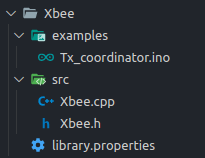
\includegraphics[scale=1]{xbee_lib.png}
\caption{ساختار فایل کتابخانه ایکس‌بی}\label{fig:xbee_lib}
\end{figure}

\subsubsection{ساختار فریم \lr{API}}

ساختار کلی فریم \lr{API} در \cref{fig:xbee_frame} \cite{Digi} نشان داده شده است. فریم با یک بایت جداکننده شروع می‌شود، سپس با ۲ بایت برای نشان‌دادن طول فریم ادامه می‌یابد و با یک بایت چک‌سام پایان می‌یابد. بایت‌های بین طول و فیلد چک‌سام را داده‌های فریم می‌نامند که برای هر نوع بسته \lr{API} متفاوت است. بایت اول فیلد طول مهم‌ترین بایت\LTRfootnote{Most Significant Byte(MSB)} و بایت بعدی کم‌اهمیت‌ترین\LTRfootnote{Least Significant Byte(LSB)} است. اولین بایت از داده‌های فریم نشان‌دهنده نوع فریم است. چک‌سام برای کمک به تست یکپارچگی داده‌ها استفاده می‌شود. اگر مقدار چک‌سام به اشتباه محاسبه شده‌باشد یا با چک‌سام واقعی داده‌های درون فریم متفاوت باشد، فریم کنار گذاشته و نادیده گرفته می‌شود.


\begin{figure}[!h]
\centering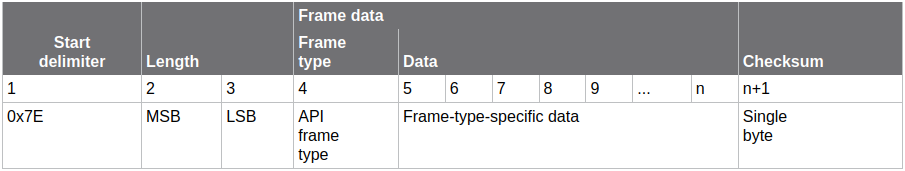
\includegraphics[scale=.65]{xbee_frame.png}
\caption{ساختار کلی فریم \lr{API} \cite{Digi}}\label{fig:xbee_frame}
\end{figure}

روش صحیح محاسبه چک‌سام فریم به شرح زیر است:
\begin{enumerate}
\item تمام بایت‌های بسته به استثنای محدودکننده شروع و طول با هم جمع می‌شوند.
\item از نتیجه فقط پایین‌ترین ۸ بیت نگه داشته می‌شود.
\item مقدار بدست‌آمده از \lr{0xFF} کم می‌شود.
\end{enumerate}

\subsubsection{فریم درخواست ارسال} \label{tx_req}

فریم‌های \lr{API} بسته به عملکردشان از چندین نوع فریم پشتیبانی می‌کنند. در این بخش فقط در مورد فریم درخواست ارسال که برای ما مهم است صحبت خواهیم کرد.

بخش‌های مختلف داده‌های فریم درخواست ارسال در \cref{tab:tx_req_frame} به همراه کاربرد آمده است.

\begin{table}[h!]
  \begin{center}
    \caption{بخش‌های مختلف داده‌های فریم درخواست ارسال \cite{Digi}}
    \label{tab:tx_req_frame}
    \begin{tabular}{|p{.1\textwidth}|p{.1\textwidth}|p{.25\textwidth}|p{.45\textwidth}|} % <-- Alignments: 1st column left, 2nd middle and 3rd right, with vertical lines in between
	   	\hline
	   	نام بخش & شماره بایت & نمونه & توضیحات\\
		\hline
	   	نوع فریم & ۳ & \lr{0x10} & بایت \lr{0x10} نشان‌دهنده فریم درخواست ارسال است.\\
		\hline
	   		   	شماره فریم & ۴ & \lr{0x01} & فریم داده را به گیرنده برای ارسال فریم وضعیت ارسال می‌شناساند. تنظیم‌کردن با مقدار ۰ پاسخ را غیرفعال می‌کند.\\
	    \hline
	   	آدرس ۶۴ بیتی مقصد & ۵ تا ۱۲ & \lr{0x0000000000000000} & آدرس ۶۴ بیتی مقصد را مشخص می‌کند.
	   	
 آدرس مقاصد خاص:
 
 	   	هماهنگ‌کننده: \lr{0x0000000000000000}
 	   	
همه‌پخشی\LTRfootnote{Broadcast}: \lr{0x000000000000FFFF}  	

نامعلوم(اگر آدرس مقصد را ندانیم): \lr{0xFFFFFFFFFFFFFFFF}
	   	\\
		\hline
	   	 	آدرس ۱۶ بیتی مقصد & ۵ تا ۱۲ & \lr{0x0000} & آدرس ۱۶ بیتی مقصد را مشخص می‌کند.
	   	
 آدرس مقاصد خاص:
 
 	   	هماهنگ‌کننده: \lr{0x0000}
 	   	

نامعلوم یا همه‌پخشی: \lr{0xFFFE}
	   	\\
		\hline
		شعاع پخش & ۱۵ & \lr{0x00} & حداکثر تعداد پرش‌هایی که انتقال همه‌پخشی می‌تواند پخش شود را تنظیم می‌کند. اگر روی ۰ تنظیم شود، شعاع پخش روی حداکثر مقدار پرش تنظیم می‌شود.\\
		\hline
		انتخاب‌ها & ۱۶ & \lr{0x00} & گزینه‌های انتقال پشتیبانی‌شده:

غیرفعال‌کردن تلاش ارسال مجدد - \lr{0x01}		

فعال‌کردن رمزگذاری \lr{APS}(با این کار حداکثر بایت‌های داده ارسالی تا ۴ بایت کاهش می‌یابد) - \lr{0x20}

استفاده از مهلت زمان طولانی برای ارسال - \lr{0x40}
		\\
		\hline
		داده ارسالی & ۱۷ به بعد & \lr{0x...} & تا ۲۵۵ بایت داده ارسالی برای مقصد\\
    	\hline
    \end{tabular}
  \end{center}
\end{table}

\subsubsection{داده ارسالی}

برای استفاده بهینه از فضای پیام در هر فریم، تصمیم گرفتیم ارتعاشات حسگر را به صورت زیر ارسال کنیم:

\begin{itemize}
\item هر داده با دقت ۳ رقم اعشار ارسال می‌شود.
\item برای جداسازی ارتعاش بر اساس محور در پیام ارسالی، از حروف \lr{x}، \lr{y} و \lr{z} استفاده نمی‌کنیم.
\item اولین بایت همیشه شناسه اندازه‌گیری را نشان می‌دهد. پس از آن پنج بایت اول نشان‌دهنده محور ایکس، پنج بایت بعدی نشان‌دهنده محور وای و پنج بایت بعدی نشان‌دهنده محور زد است. هر داده در پنج بایت نمایش داده می‌شود، برای مثال عدد ۴۵۲/۳- بصورت \lr{\{'-','3','4','5','2'\}} نمایش داده می‌شود.
\end{itemize}

در سمت گیرنده، داده‌ها باید به حالت اولیه تبدیل شوند.

\subsubsection{فایل \lr{Xbee.cpp} و توابع مهم}

برای تنظیم آدرس مقصد برای هر فریم کلاس \lr{XbeeDestAddress} را تعریف کرده‌ایم. این کلاس شامل فیلد ۶۴ بیتی و ۱۶ بیتی برای آدرس است. با توجه به اینکه به آرایه‌ای از بایت‌ها برای تشکیل فریم نیاز داریم، توابعی متناظر برای گرفتن هر یک از فیلدها نیز نوشته شده است.


برای تشکیل فریم درخواست انتقال کلاس \lr{XbeeRequest} تعریف شده است. تابع \lr{constructFrame} برای ایجاد فریم با استفاده از شناسه فریم و داده مورد نظر نوشته شده است. این تابع فریم را طبق \cref{tx_req} ایجاد کزده و فریم تشکیل‌شده برگردانده می‌شود. با استفاده از تابع \lr{writeFrameToSerial} نیز می‌توان فریم تشکیل‌شده را بر روی درگاه سریال دلخواه نوشت.

\subsection{‫ﺧﻮﺍﺑﻴﺪﻥ‬ ‫ﻭ‬ ‫ﺑﻴﺪﺍﺭﺷﺪﻥ‬ ‫ﺩﺭ‬ ‫ﺑﺎﺯﻩ‬‌‫ﻫﺎی ‬‫ﺯﻣﺎﻧﻲ‬ ‫ﻣﺸﺨﺺ‬}

برای کاهش مصرف انرژی، حسگر تنها در زمان‌های مشخص لرزش را احساس می‌کند. در سایر زمان‌ها بورد آردوینو برای کاهش مصرف انرژی به خواب می‌رود. برای این کار از کتابخانه \lr{LowPower.h} استفاده می‌کنیم. با استفاده از تابع \lr{powerDown} آردوینو به خواب می‌رود. برای بیدارشدن در زمان مشخص، آردوینو از زمان‌بند داخلی خود\LTRfootnote{Watchdog Timer} استفاده می‌کند. اما این تایمر بعد از ۸ ثانیه سرریز شده و بورد بیدار می‌شود. برای زمان‌های بیشتر باید به محض بیدارشدن مجدد تا رسیدن به زمان مورد نظر، آن را مجددا به خواب ببریم. این کار در تابع \lr{longSleep} انجام شده است.

\section{دروازه}

در دروازه ما از زبان برنامه‌نویسی پایتون برای دریافت فریم‌های زیگبی، ذخیره‌کردن و ارسال داده‌ها به سرور مرکزی پس از رسیدن به آستانه استفاده می‌کنیم. ساختار پروژه دروازه در \cref{fig:gateway_structure} نشان داده شده است. در این بخش به بررسی هر یک از فایل ها می‌پردازیم.


\begin{figure}[!h]
\centering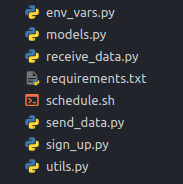
\includegraphics[scale=1]{gateway_structure.png}
\caption{ساختار پروژه دروازه}\label{fig:gateway_structure}
\end{figure}

\subsection{فایل \lr{env\_vars.py}}

این فایل از بسته \lr{load\_dotenv} برای خواندن متغیرهای محیطی استفاده می‌کند. برخی از این متغیرها برای برقراری ارتباط با سرور استفاده می‌شوند مانند شماره پورت سرور و آیپی سرور. سایر آنها برای برقراری ارتباط با دستگاه ایکس‌بی استفاده می‌شوند. این متغیرهای محیطی به عنوان متغیرهای پایتون تنظیم می‌شوند و سپس در ماژول‌های دیگر پایتون استفاده می‌شوند.

\subsection{فایل \lr{models.py}}

در این فایل ما سه کلاس برای نمایش داده‌های ارتعاش، اندازه گیری‌ها و هر گره انتهایی تعریف کرده‌ایم.

کلاس داده ارتعاش شامل داده‌های لرزش در سه محور ثبت‌شده توسط حسگر می‌باشد. هر اندازه‌گیری بسته به فرکانس نمونه‌برداری شامل چندین داده ارتعاش است. همچنین شامل یک شناسه و زمانی است که اندازه‌گیری در آن انجام شده است. از آنجایی که برای برقراری ارتباط داده‌های ارتعاش با زیگبی قطعه‌بندی\LTRfootnote{Fragmentation} لازم است و زمانی بین ارسال هر فریم لازم است، تابع \lr{thread\_handler} تعریف شده است تا در صورت اتمام زمان اتصال یا از بین رفتن برخی فریم‌ها، اندازه‌گیری از داده‌های دریافتی قبلی بطور خودکار تکمیل شود. پس از آن داده‌های جدید ذخیره می‌شوند.

هر گره دارای یک شناسه است که با شناسه فرستنده ارائه‌شده در هر فریم زیگبی مشخص می‌شود. همچنین هر گره شامل چندین اندازه‌گیری است. هنگامی که اندازه‌گیری جدیدی به لیست اندازه‌گیری‌ها اضافه می‌شود، زمان‌بند رشته‌ای\LTRfootnote{Thread Timer} با دوره وقفه مشخص و تابع \lr{thread\_handler} شروع می‌شود.

\subsection{فایل \lr{receiver.py}}

در این فایل سروری تعریف می‌کنیم که بطور بی‌نهایت به درگاه \lr{USB} متصل به دستگاه ایکس‌بی گوش می‌دهد. برای خواندن داده‌ها و استخراج داده هر فریم از کتابخانه \lr{digi-xbee} استفاده می‌کنیم. برای مقداردهی اولیه یک نمونه ایکس‌بی، درگاه و نرخ باود\LTRfootnote{Buad Rate} ارتباط لازم است. در تابع \lr{decode\_sensor\_data}، شناسه اندازه‌گیری و داده‌های ارتعاش را استخراج می‌کنیم. در تابع \lr{receive}، به منتظر دریافت پیام جدید می‌مانیم. داده‌های پیام را به گره و اندازه‌گیری مربوطه اضافه می‌کنیم و سپس داده‌های ذخیره‌شده را بروز می‌کنیم.

\subsection{فایل \lr{requirements.txt}}

این فایل برای تعیین بسته‌ها، نسخه‌ها و وابستگی‌های لازم استفاده می‌شود. سپس از این فایل برای نصب بسته‌های مشخص‌شده با مدیریت بسته پایتون پیپ\LTRfootnote{pip} استفاده می‌شود.

\subsection{فایل \lr{schedule.sh}}

آستانه تعریف‌شده بر اساس زمان است. این اسکریپت در کنار گیرنده اجرا می‌شود. در این اسکریپت یک کار \lr{crontab} برنامه‌ریزی می‌شود که هر ۱۵ دقیقه اجرا شود. این زمان‌بندی با استفاده از علامت \lr{*/15 * * * *} انجام می‌شود که به معنای اجرای اسکریپت ارسال داده پایتون در هر دقیقه قابل‌تقسیم بر ۱۵ است.

\subsection{فایل \lr{send\_data.py}}

در این فایل اطلاعات ذخیره‌شده در حافظه بارگذاری می‌شود. برای سرور و فراخوانی نقاط انتهایی \lr{API} از کتابخانه \lr{requests} استفاده می‌کنیم. برای دریافت رمز احراز هویت \lr{JWT} برای ارسال داده‌های ارتعاشی، یک درخواست پست با آدرس مک دستگاه و رمز عبور به سرور ارسال می‌شود تا رمز احراز هویت را دریافت کند. پس از آن داده‌های لرزش فرمت‌شده بصورت جیسان\LTRfootnote{JavaScript Object Notation(JSON)} در بدنه درخواست به همراه هدر احراز هویت به سرور ارسال و فایل ذخیره نیز پاک می‌شود.

\subsection{فایل \lr{signup.py}}

این فایل برای ثبت دروازه در سرور با رمز عبور و آدرس مک مربوطه استفاده می‌شود.

\subsection{فایل \lr{utils.py}}

این فایل شامل برخی از توابع کاربردی مانند دریافت آدرس مک دستگاه، دریافت زمان جاری در شکل مورد نظر، بروز رسانی داده‌های ذخیره‌شده و تعریف کلاس مدل جیسان برای کد‌کردن داده‌ها می‌باشد.

\section{پیش‌پردازش}

داده‌های جمع‌آوری‌شده از حسگر در هر سه محور می‌توانند تحت تاثیر شتاب گرانش زمین باشند. همچنین شتاب اندازه‌گیری‌شده توسط حسگرهای کم‌هزینه \lr{MEMS} نیز اکثرا تحت تاثیر یک مقدار غیرصفر دچار انحرافاتی می‌شوند که منجر به افزایش یا کاهش اندازه‌گیری‌ها می‌شود\cite{jung2017vibration}. برای حذف انحرافات و شتاب گرانش ناخواسته، داده‌ها را در مرحله پیش‌پردازش هنجارسازی می‌کنیم. برای حذف ناهنجاری‌ها مطابق \cref{form:norm} میانگین هر محور را ار هر داده کم می‌کنیم. لازم به ذکر است که $\hat{a}^l_{nm}$ نماد ماتریس هنجارشده برای شتاب در سه محور، گره \lr{n} و اندازه‌گیری \lr{m}ام است.

\begin{equation}
\label{form:norm}
\hat{a}^l_{nm}=a^l_{nm}-\sum_{k=1}^K \dfrac{a^l_{nmk}}{K}
\end{equation}

\section{پایگاه داده سری زمانی}

مدل داده \lr{InfluxDB} داده‌های سری زمانی را در سطل‌ها\LTRfootnote{Buckets} و اندازه‌گیری‌ها سازماندهی می‌کند. یک سطل می‌تواند چندین اندازه‌گیری داشته باشد. اندازه‌گیری گروه‌بندی منطقی برای داده‌های سری زمانی است که شامل چندین برچسب\LTRfootnote{Tag} و فیلد است. همه نقاط در یک اندازه‌گیری معین باید برچسب‌های یکسانی داشته باشند. برچسب‌ها جفت‌های کلید-مقدار با مقادیری متفاوت هستند که اغلب تغییر نمی‌کنند و برای ذخیره ابرداده\LTRfootnote{Meta data} برای هر نقطه در نظر گرفته شده‌اند. فیلدها جفت‌های کلید-مقدار هستند که مقادیر آنها در طول زمان تغییر می‌کنند. زمان مرتبط با داده‌ها نیز ذخیره می‌شوند و هنگام پرس‌وجو داده‌ها برحسب آن مرتب می‌شوند\cite{influx_doc}.


برای ارتباط با پایگاه داده از کلاینت پایتون \lr{influxDB} استفاده می‌کنیم. برای شروع یک اتصال به نام سطل، سازمان، نشانه و نشانی نیاز داریم. برای نوشتن داده‌ها از تابع \lr{write\_api} و برای پرس‌وجوی داده‌ها در پایگاه داده از \lr{query\_api} استفاده می‌کنیم.


برای نوشتن داده‌ها باید نقاطی را که می‌خواهیم اضافه کنیم، مشخص کنیم. نقطه یک داده واحد است که با اندازه‌گیری، کلیدهای برچسب، مقادیر برچسب، کلید فیلد و زمان مشخص می‌شود. برای پرس‌وجوی داده‌ها، از عملگر لوله جلو\LTRfootnote{Pipe-Forward(|>)} برای اتصال خروجی یک تابع بعنوان ورودی تابع بعدی استفاده می‌کند\cite{influx_doc}. سه تابع اصلی برای پرس‌وجوکردن داده‌ها وجود دارد:

\begin{itemize}
\item \lr{from()}: داده‌ها را از یک سطل جستجو می‌کند.
\item \lr{range()}: داده‌ها را بر اساس محدوده‌ی زمانی فیلتر می‌کند. برای جستجو به پرس‌وجوهای محدود به یک بازه‌ی زمانی خاص نیاز داریم.
\item \lr{filter()}: داده‌ها را بر اساس مقادیر ستون فیلتر می‌کند. هر سطر با \lr{r} و هر ستون با ویژگی \lr{r} نشان داده می‌شود. می‌توان چند فیلتر متوالی اعمال کرد.
\end{itemize}

تابع دیگری که استفاده کرده‌ایم \lr{pivot()} است که برای تبدیل داده‌ها به یک طرح رابطه‌ای\LTRfootnote{Relational Schema} بر اساس زمان استفاده می‌شود.

\subsection{ساختار کلی}

ساختار کلی پایگاه داده طراحی‌شده در این پروژه در \cref{fig:influx_structure} نشان داده شده است. هر یک از ویژگی‌های استخراج‌شده در سمت چپ در اندازه‌گیری‌های مختلف قرار گرفته‌اند. در وسط تصویر نیز برچسب‌ها که بین همه اندازه‌گیری‌ها مشترک است قرار گرفته است. در سمت راست تصویر نیز فیلدهای هر اندازه‌گیری آورده شده است. در ادامه به توضیح توابع نوشتن و پرس‌وجوی اندازه‌گیری‌ها می‌پردازیم.


\begin{figure}[!h]
\centering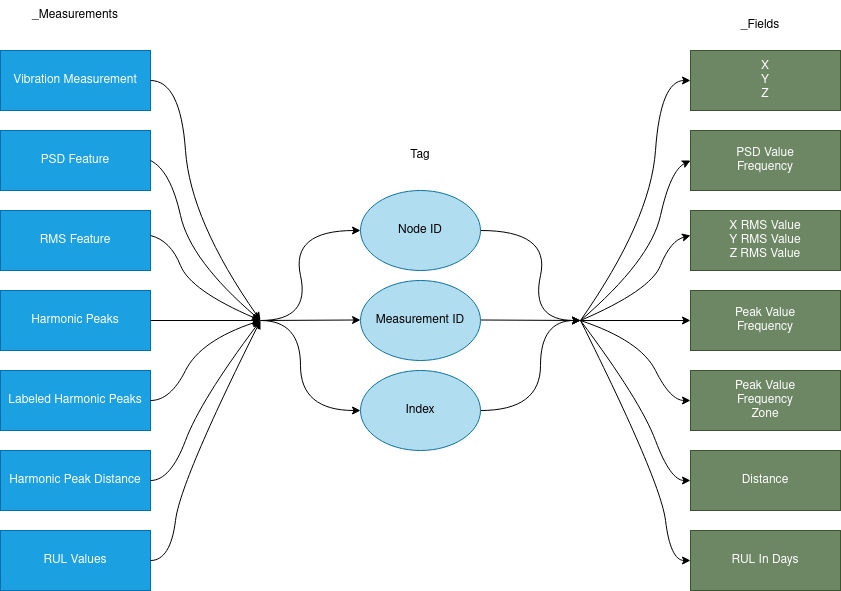
\includegraphics[scale=.5]{influx_structure.png}
\caption{ساختار کلی پایگاه داده سری زمانی}\label{fig:influx_structure}
\end{figure}

\subsection{اندازه‌گیری‌ها و توابع مربوط به نوشتن و گرفتن داده}

در هر اندازه‌گیری، فیلدهای مربوط را ذخیره می‌کنیم. فیلدهای هر داده ثبت می‌شود و با یک گره و یک اندازه‌گیری همراه است. همچنین یک شماره به هر نمونه در اندازه‌گیری بعنوان شناسه داده می‌شود.

برای نوشتن داده‌ها در پایگاه داده توابع \lr{write\_\$\{measurement name\}} پیاده‌سازی شده است که یک نقطه جدید برای هر داده با شناسه اندازه‌گیری، شناسه گره و شماره بعنوان برچسب و فیلدهای مربوطه ایجاد می‌کند.

برای پرس‌وجوی داده، توابع \lr{get\_\$\{measurement name\}} پیاده‌سازی شده است. پرس‌وجو بگونه‌ای نوشته شده است که اگر شناسه اندازه‌گیری یا شناسه گره ارائه شود، فقط داده‌های مرتبط برگردانده می‌شود. در هر پرس‌وجو، ما تمام داده‌ها را از اندازه‌گیری مربوط انتخاب می‌کنیم و در صورت وجود شناسه گره یا اندازه‌گیری فیلتر می‌کنیم. سپس زمان فیلدها، مقادیر آنها و برچسب‌ها را نگه می‌داریم و از تابع \lr{pivot} برای تبدیل نتایج به طرح رابطه‌ای استفاده می‌کنیم. بعنوان نمونه، کد پرس‌وجوی \lr{vibration\_measurement} در \cref{fig:vm_query} نشان داده شده است.

\begin{figure}[!h]
\centering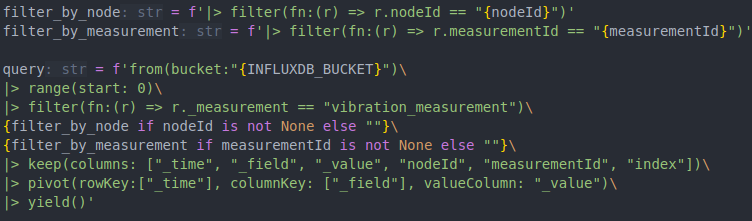
\includegraphics[scale=.75]{vm_query.png}
\caption{کد پرس‌وجوی \lr{vibration\_measurement}}\label{fig:vm_query}
\end{figure}

\subsection{توابع گرفتن شناسه گره و اندازه‌گیری}

در این توابع برای گرفتن شناسه‌ها به تنهایی، برچسب مورد نظر را نگه می‌داریم و جهت جلوگیری از تکرار با استفاده از تابع \lr{unique()} مقادیر یکتای شناسه را برمی‌گردانیم.

\subsection{تابع \lr{get\_starting\_service\_date}}

این تابع برای دریافت زمان اولین داده ثبت‌شده بعنوان مبدا زمانی برای محاسبه زمان سرویس‌شدن تجهیزات نوشته شده است.

\subsection{تابع حذف داده‌ها و حافظه پنهان}

برای حذف از کلاس \lr{DeleteApi} کتابخانه استفاده می‌کنیم. جهت حذف حافظه پنهان، همه اندازه‌گیری‌ها را، بجز آنهایی که خودمان تعریف کرده‌ایم، تا زمان فعلی حذف می‌کنیم. همچنین برای حذف همه داده‌ها با استفاده از تابع \lr{clear\_vibration\_data}، همه اندازه‌گیری‌ها را حذف می‌کنیم.

\section{برنامه وب و چارچوب ویو}

وظایف مختلفی در توسعه‌ی یک برنامه وب سمت کاربر وجود دارد. بسته‌های زیادی برای بخشی خاص توسعه داده شده‌اند تا کار توسعه برنامه آسان‌تر شود. در این پروژه علاوه بر استفاده از چارچوب ویو، از کتابخانه‌ها و ماژول‌های دیگر برای کارهای مختلف استفاده کرده‌ایم. در این قسمت در مورد کتابخانه‌های مهم استفاده‌شده، ساختار فایل پروژه و اجزای اصلی برنامه صحبت و تصاویری از محیط پیاده‌سازی‌شده را مشاهده می‌کنیم.

\subsection{کتابخانه‌ها و ماژول‌ها}

\subsubsection{چارچوب ناکست}

ناکست\LTRfootnote{Nuxt} یک چارچوب توسعه وب سطح بالای نودجی‌اس\LTRfootnote{Node.js} برای ایجاد برنامه‌های ویو است که می‌تواند در دو حالت مختلف برنامه جهانی\LTRfootnote{Universal(SSR)} و تک‌صفحه‌ای\LTRfootnote{Single Page Application(SPA)} توسعه و استقرار یابد. علاوه بر این، می‌توان این دو نوع را در ناکست بعنوان برنامه‌های تولیدشده ایستا\LTRfootnote{Static} مستقر کرد. قدرت کامل ناکست در حالت جهانی یا تفسیر سمت سرور نهفته است. ناکست بر روی ویو ایجاد شده است و دارای ویژگی‌های اضافی مانند داده‌های ناهمزمان، میان‌افزار، طرح‌بندی، ماژول‌ها و افزونه‌ها است که برنامه را ابتدا در سمت سرور و سپس در سمت کلاینت اجرا می‌کند. در این حالت برنامه معمولاً سریع‌تر از برنامه‌های سنتی سمت سرور ارائه می‌شود\cite{kok2020hands}. ناکست ساختار فایل ساده‌ای نیز دارد که توسعه برنامه وب را بسیار ساده‌تر می‌کند که در بخش بعدی در مورد آن توضیح می‌دهیم.


\subsubsection{کتابخانه ویوتیفای}

ویوتیفای\LTRfootnote{Vuetify} یک چارچوب کامل رابط کاربری است که بر روی ویو ساخته شده است. هدف این پروژه ارائه ابزارهای مورد نیاز توسعه‌دهندگان برای ایجاد تجربیات کاربر غنی و جذاب است. برخلاف سایر چارچوب‌ها، ویوتیفای از ابتدا به گونه‌ای طراحی شده است که یادگیری آن آسان است و صدها مؤلفه با دقت ساخته‌شده از مشخصات طراحی مادی\LTRfootnote{Material Design} همراه آن است\cite{vuetify}.

ویوتیفای برای طراحی از یک رویکرد اول تلفن همراه\LTRfootnote{Mobile First} استفاده می‌کند، به این معنی که برنامه وب به‌سادگی و بدون بهم‌ریختگی روی تلفن همراه، تبلت یا رایانه اجرا می‌شود. ویوتیفای را می‌توان به‌سادگی بعنوان یک ماژول به ناکست اضافه و در پروژه استفاده کرد\cite{vuetify}.


\subsubsection{کتابخانه چارت}

در ابن پروژه چندین داده تحلیلی داریم که با استفاده از نمودارها قابل مشاهده هستند. برای این کار از کتابخانه چارت‌\LTRfootnote{Chart.js} استفاده کرده‌ایم. کتابخانه چارت مجموعه‌ای از انواع نمودارها، افزونه‌ها و گزینه‌های سفارشی‌سازی را ارائه می‌دهد. علاوه بر مجموعه‌ای معقول از انواع نمودار داخل کتابخانه، می‌توان از انواع نمودارهای توسعه‌داده‌شده توسط جامعه نیز استفاده کرد. علاوه بر این، می‌توان چندین نوع نمودار را در یک نمودار ترکیبی قرار داد. این کتابخانه با افزونه‌های سفارشی ایجاد حاشیه‌نویسی، بزرگنمایی یا قابلیت کشیدن و رهاکردن را ممکن ساخته است\cite{chart}.

\subsubsection{کتابخانه اکسیوس}

اکسیوس\LTRfootnote{Axios} یک سرویس گیرنده \lr{HTTP} مبتنی بر وعده\LTRfootnote{Promise} برای نودجی‌اس و مرورگر است که می‌تواند در هر دو با پایگاه کد مشابه اجرا شود. این کتابخانه در سمت سرور از ماژول اصلی \lr{HTTP} نودجی‌اس و در مرورگر از \lr{XMLHttpRequests} استفاده می‌کند. مزیت اصلی این کتابخانه سادگی در ارسال درخواست‌های مختلف، دریافت پاسخ آنها و پشتیبانی از \lr{API} وعده است\cite{axios}. همچنین می‌توان آن را بعنوان یک ماژول به پروژه ناکست اضافه کرد.

\subsubsection{ماژول احراز هویت ناکست}

احراز هویت بخش بسیار مهمی از هر برنامه وب است که شامل مراحل زیر است:

\begin{itemize}
\item ارسال اطلاعات کاربران به سرور جهت تایید
\item دریافت و ذخیره توکن احراز هویت
\item استفاده از آن توکن برای تماس های بعدی \lr{API}
\end{itemize}

این ماژول با استفاده از یک طرح احراز هویت قابل‌تنظیم یا با استفاده از یکی از ارائه‌دهندگان مستقیم پشتیبانی‌شده، احراز هویت کاربران را تأیید می‌کند و یک \lr{API} برای احراز هویت و دسترسی به اطلاعات کاربر فراهم می‌کند. در حالیکه این ماژول ذخیره اطلاعات در سمت کاربر را بر عهده دارد، مدیریت جلسه یا احراز هویت مبتنی بر جلسه در سمت سرور را ارائه نمی‌کند\cite{nuxt_auth}.

\subsection{ساختار پروژه}

ساختار پروژه در \cref{fig:front_structure} نشان داده شده است. برخی از فایل‌ها و پوشه‌ها بخشی از چارچوب ناکست هستند.

\begin{figure}[!h]
\centering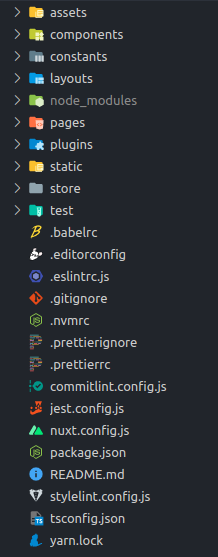
\includegraphics[scale=.75]{front_structure.png}
\caption{ساختار پروژه برنامه وب}\label{fig:front_structure}
\end{figure}

برخی دیگر از این فایل‌ها مانند \lr{eslint} برای هشدار در مواقعی که کد نوشته‌شده مطابق قواعد تعریف شده نباشد استفاده می‌شود، برخی دیگر مانند \lr{style lint} برای داشتن سبکی یکپارچه و تمیز در بین همه فایل‌ها و توسعه‌دهندگان استفاده می‌شوند.

همچنین چند فایل وجود دارد که بسته‌های لازم، نسخه‌های آنها و همچنین چند اسکریپت برای اجرای پروژه را مشخص می‌کنند. مدیریت‌کننده بسته مورد استفاده در این پروژه یارن\LTRfootnote{Yarn} نام دارد. در فایل \lr{yarn.lock} نسخه‌های دقیق بسته‌ها و وابستگی‌های آنها توسط یارن مشخص شده است و از آن برای سریع و قابل‌اعتمادبودن تفکیک وابستگی‌ها استفاده می‌کند. در فایل \lr{package.json} اسکریپت‌ها، وابستگی‌ها و وابستگی‌های زمان توسعه مشخص شده‌اند. این فایل برای شناسایی بسته‌های لازم توسط یارن در اولین اجرا لازم است.

\subsubsection{پوشه \lr{assets}}

این پوشه شامل فایل‌های تفسیرنشده مثل استایل‌ها\LTRfootnote{Styles}، تصاویر و فونت‌ها است\cite{nuxt}.

\subsubsection{پوشه \lr{components}}

این پوشه حاوی مؤلفه‌های ویو است. مؤلفه‌ها بخش‌های مختلف صفحه را تشکیل می‌دهند و می‌توانند دوباره استفاده شوند و در صفحات، طرح‌بندی‌ها\LTRfootnote{Layouts} و حتی سایر مؤلفه‌ها قرار گیرند\cite{nuxt}.

\subsubsection{پوشه \lr{layouts}}

برای تغییر ظاهر برنامه، طرح‌بندی‌ها کمک بزرگی هستند. این تغییر می‌تواند افزودن نوار کناری\LTRfootnote{Sidebar} یا طرح‌بندی‌های متفاوت برای تلفن‌همراه و رایانه باشد. در این پروژه دو طرح‌بندی پیش‌فرض و خطا وجود دارد\cite{nuxt}.

\subsubsection{پوشه \lr{pages}}

این پوشه شامل نماها و مسیرهای برنامه است. ناکست تمام فایل‌های \lr{.vue} داخل این پوشه را می‌خواند و بطور خودکار پیکربندی مسیریاب را ایجاد می‌کند\cite{nuxt}.

\subsubsection{پوشه \lr{plugins}}

این پوشه شامل افزونه‌های جاوا اسکریپت است که می‌خواهیم قبل از نمونه‌سازی ریشه برنامه اجرا کنیم\cite{nuxt}. در این پروژه برای ایجاد مؤلفه نمودارها و همینطور دخالت در درخواست‌های اکسیوس و مدیریت خطاهای مربوط به آن افزونه‌هایی نوشته‌ایم.

\subsubsection{پوشه \lr{statics}}

این پوشه بطور مستقیم به ریشه سرور نگاشت می‌شود و حاوی فایل‌هایی است که تغییر نخواهند کرد. همه فایل‌های ارائه‌شده بطور خودکار توسط ناکست ارائه\LTRfootnote{Serve} می‌شوند و از طریق آدرس ریشه پروژه قابل دسترسی هستند\cite{nuxt}.

\subsubsection{پوشه \lr{store}}

گاهی اوقات در پروژه به اطلاعات مشترک و قابل دسترسی بین همه مؤلفه‌ها نیاز داریم. یکی از راهکارهای این مسئله استفاده از سیستم ذخیره‌سازی مرکزی است که در آن یک بخش داده‌های مشخص‌شده و تغییراتشان را مدیریت می‌کند. در ویو این مسئولیت بر عهده ویوایکس\LTRfootnote{Vuex} است. این پوشه شامل فایل‌های ویوایکس است. ویوایکس همراه ناکست و بصورت خارج از جعبه\LTRfootnote{Out of the Box} عرضه می‌شود اما بطور پیش‌فرض غیرفعال است. ایجاد یک فایل \lr{index.js} در این پوشه، ویوایکس را فعال می کند\cite{nuxt}. در این پروژه برای نگهداری مشخصات ظاهری و مدیریت ورود کاربران از ویوایکس استفاده می‌کنیم.

\subsubsection{فایل \lr{nuxt.config.js}}

بطور پیش‌فرض، ناکست برای پوشش بیشتر موارد استفاده پیکربندی شده است. این پیکربندی پیش‌فرض ناکست و ماژول‌های آن را می‌توان با فایل \lr{nuxt.config.js} بازنویسی کرد\cite{nuxt}. بازنویسی‌های ما شامل افزودن برچسب‌های ابرداده، مشخص‌کردن ماژول‌ها، افزودنی‌ها و استایل کلی و پیکربندی برخی ماژول‌ها مانند ماژول احراز هویت(برای مشخص‌کردن روش احراز هویت، مسیرهای حفاظت‌شده و آدرس سرور برای تاید احراز هویت) و ویوتیفای(برای مشخص‌کردن ظاهر صفحات و رنگ‌ها) است.

\subsection{مؤلفه‌های اصلی}

در این بخش در مورد اجزای اصلی و برخی از صفحات این پروژه صحبت خواهیم کرد.


\subsubsection{کارت خلاصه}

در این مؤلفه، آمار خلاصه همه موارد مختلف را نشان می‌دهیم. عنوان، خلاصه و نماد بعنوان ورودی\LTRfootnote{Props} ارائه می‌شوند و به‌سادگی با تکرار روی هر مورد نشان داده می‌شوند. نتایج را می‌توان در \cref{fig:summary_card} مشاهده کرد که آمار کاربران، گره‌ها و دروازه‌ها را نشان می‌دهد.

\begin{figure}[!h]
\centering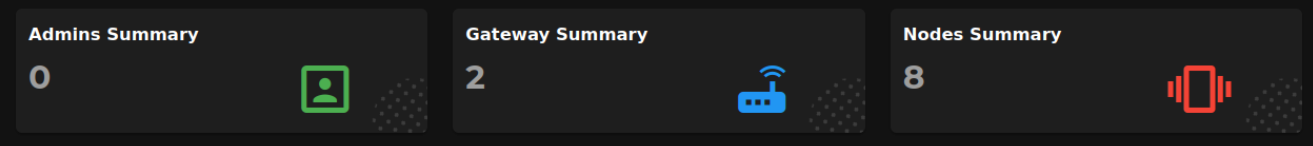
\includegraphics[scale=.45]{summary_card.png}
\caption{مؤلفه کارت خلاصه}\label{fig:summary_card}
\end{figure}

\subsubsection{فرم‌ها}

تمامی اجزای مربوط به فرم‌ها در این پوشه قرار دارند. مؤلفه ورود دارای دو فیلد متنی برای ایمیل و رمز عبور کاربران است. هنگامی که کاربر بر روی دکمه ورود کلیک می‌کند، معتبربودن ایمیل و رمز عبور بررسی می‌شود. سپس درخواست مجوز برای کاربر به سرور ارسال می‌شود و در صورت صحیح‌بودن اطلاعات، کاربر به صفحه اصلی هدایت می‌شود. در غیر این صورت، پیام خطای مناسب با مولفه اسنک‌یار\LTRfootnote{SnackBar} نمایش داده می‌شود. در \cref{fig:login_page} صفحه ورود با پیام خطای نادرستی رمز عبور نشان داده شده است.

\begin{figure}[!h]
\centering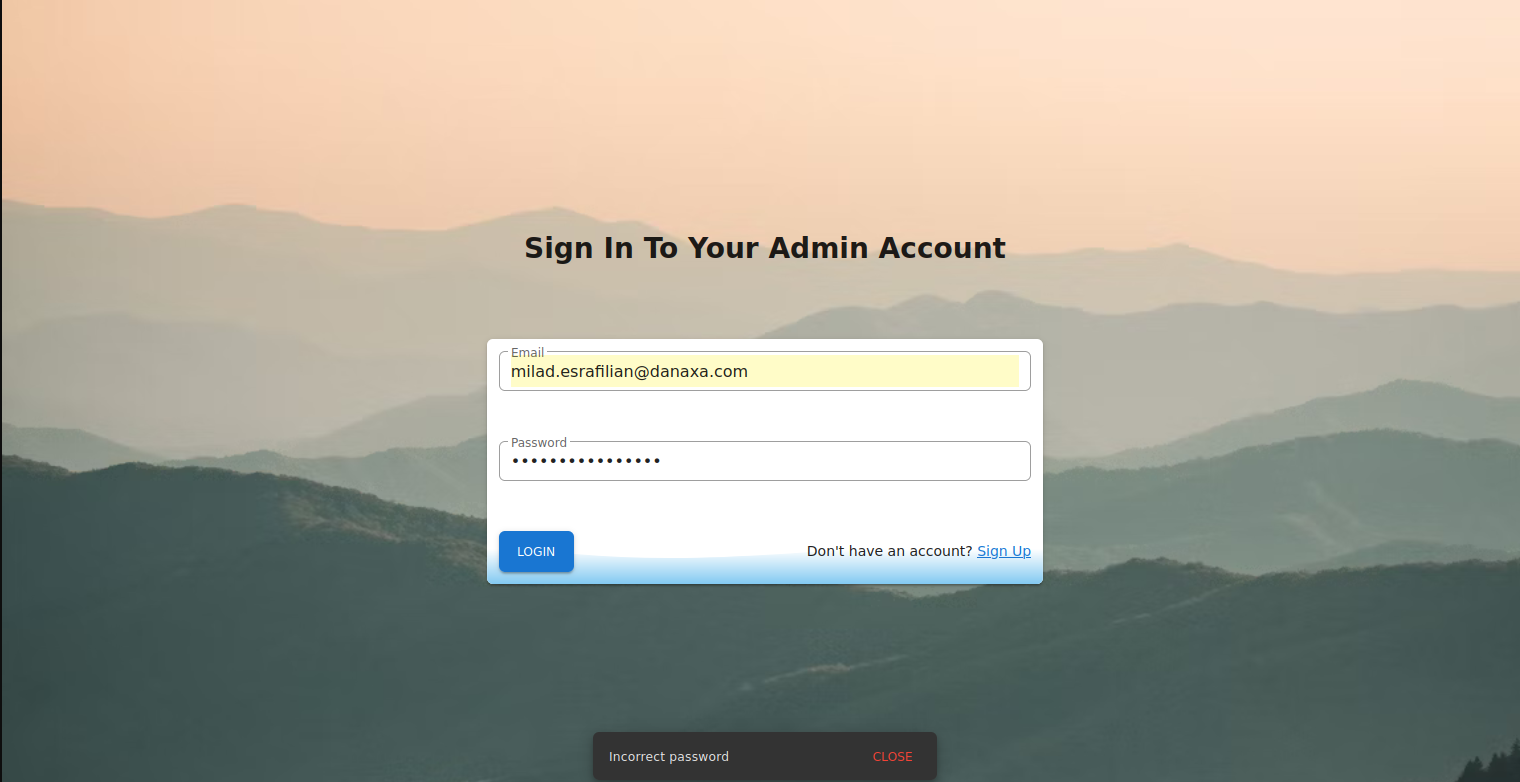
\includegraphics[scale=.38]{login_page.png}
\caption{صفحه ورود و پیغام خطای رمز عبور نادرست}\label{fig:login_page}
\end{figure}

همین روند در مؤلفه ثبت‌نام طی می‌شود، با این تفاوت که یک فیلد نام نیز در آن وجود دارد که در \cref{fig:signup_page} قابل مشاهده است.

\begin{figure}[!h]
\centering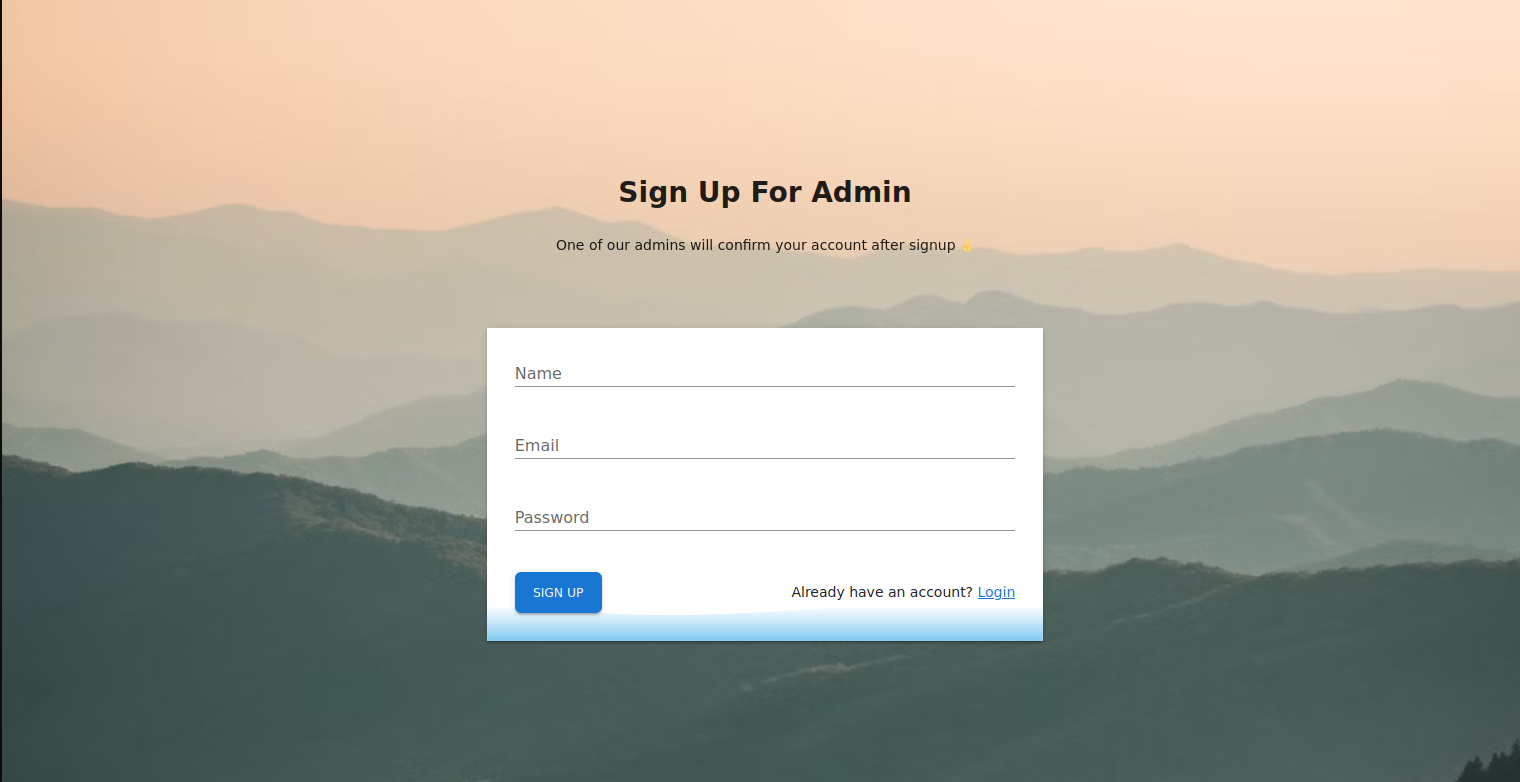
\includegraphics[scale=.38]{signup_page.png}
\caption{صفحه ثبت‌نام کاربر جدید}\label{fig:signup_page}
\end{figure}

\subsubsection{اسنک‌بار}

مؤلفه اسنک‌بار برای نمایش پیام‌های خطا استفاده می‌شود. پیغام خطا به عنوان ورودی به آن داده می‌شود. اسنک‌بار را می‌توان با فشردن دکمه بستن بست.


\subsubsection{فوتر}

فوتر\LTRfootnote{Footer} در پایین تمام صفحات نشان داده می‌شود و شامل تاریخ و پیام کپی‌رایت\LTRfootnote{Copy Right} است.

\subsubsection{مؤلفه‌های \lr{GatewayDetail} و \lr{UserDetail}}

این دو مولفه بسیار شبیه بهم هستند اما اطلاعات متفاوتی را درباره کاربران و دروازه‌ها نشان می‌دهند. هر کاربر و دروازه باید پس از ثبت‌نام توسط مدیر دیگری تایید شود. این کار را می‌توان با تغییر کلید تایید در صفحات مرتبط انجام داد. \cref{fig:gateway_page} دو دروازه فعال تاییدشده را نشان می‌دهد. پس از تایید کاربر یا دروازه، کلید غیرفعال می‌شود.

\begin{figure}[!h]
\centering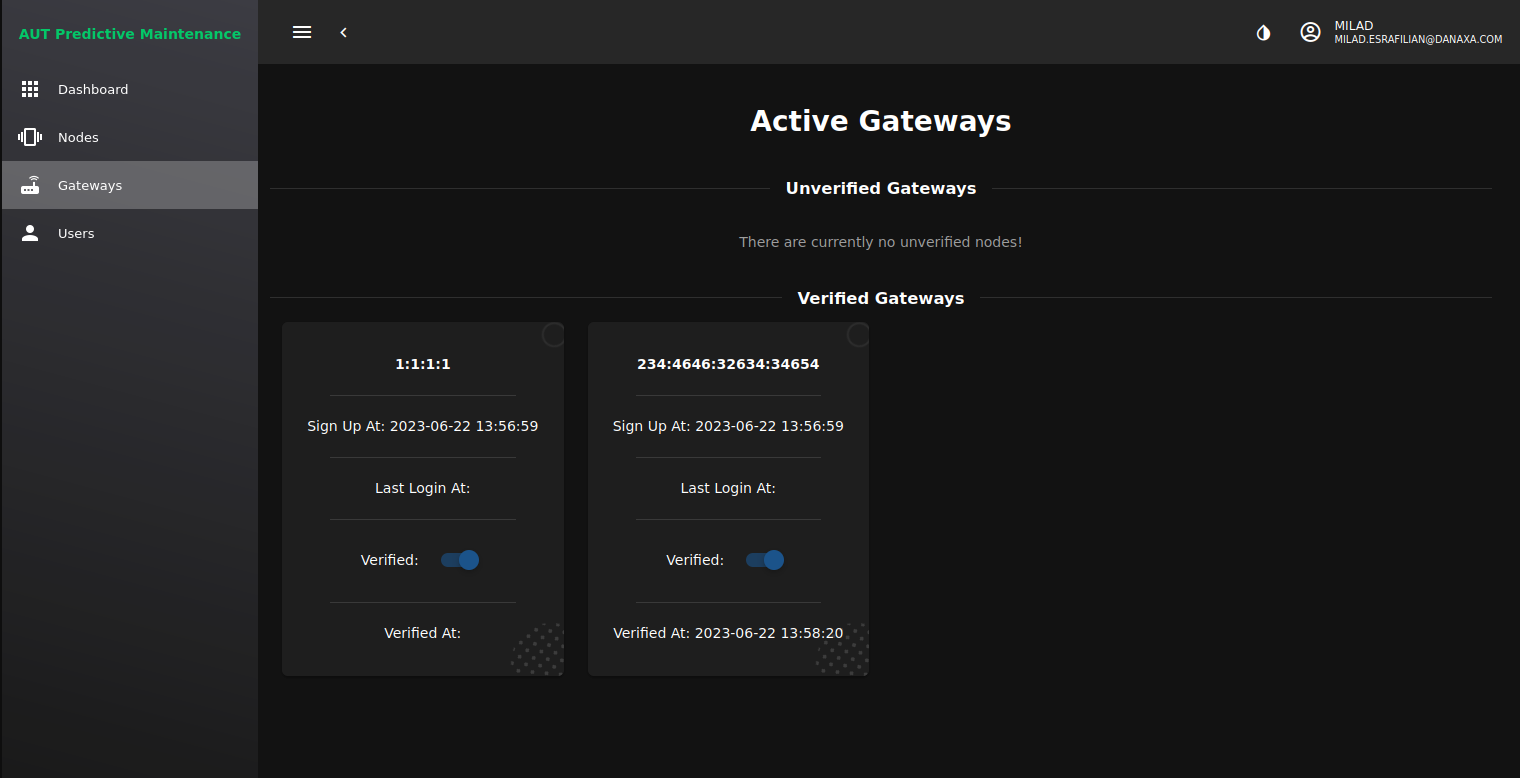
\includegraphics[scale=.38]{gateway_page.png}
\caption{صفحه دروازه‌های فعال}\label{fig:gateway_page}
\end{figure}

\subsubsection{داشبورد}

داشبورد\LTRfootnote{Dashboard} یک نمای کلی از ادمین‌های فعال، دروازه‌ها و گره‌ها ارائه می‌دهد. همچنین در این صفحه می‌توانیم به هر گره مطابق \cref{fig:dashboard} دسترسی داشته باشیم.

\begin{figure}[!h]
\centering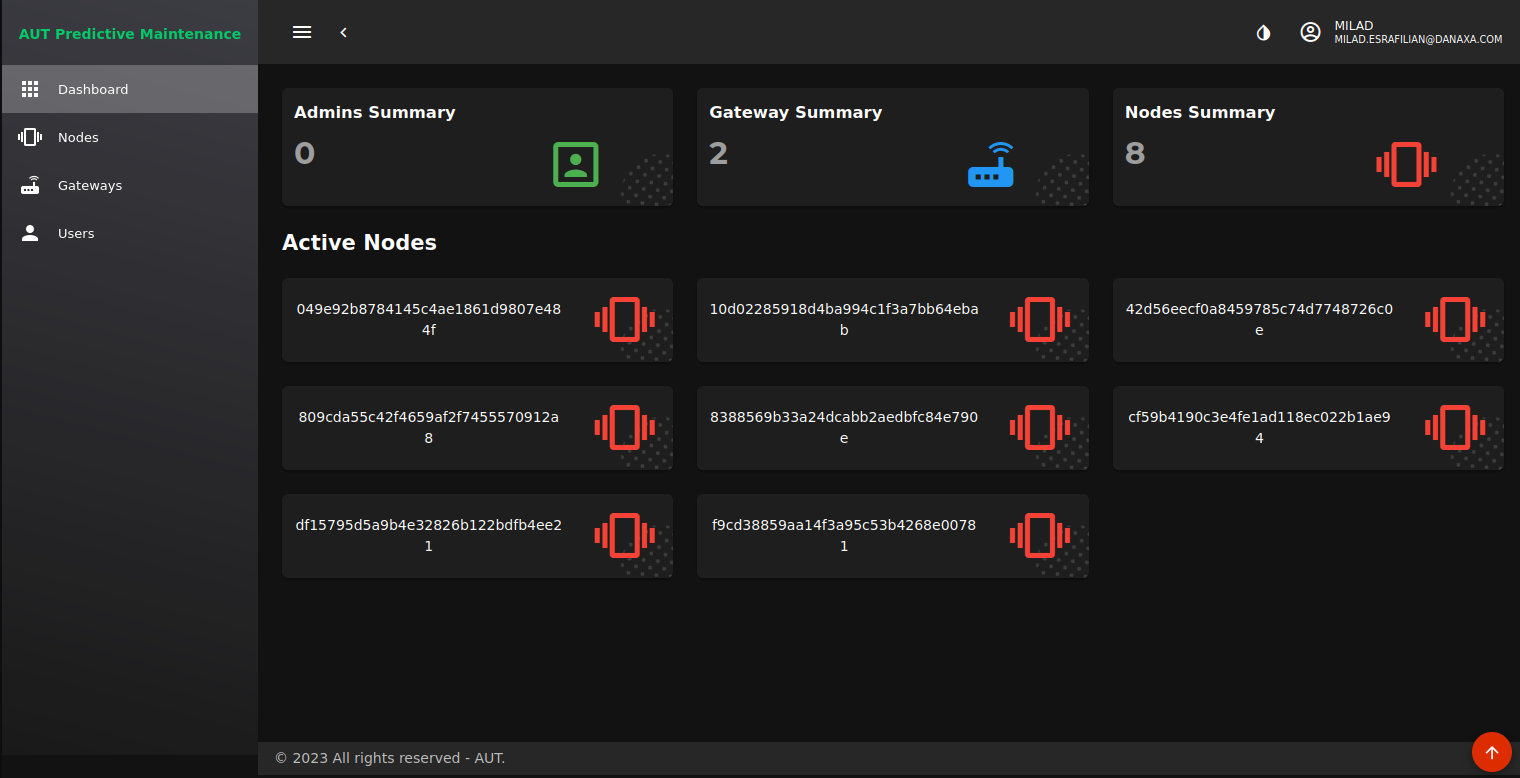
\includegraphics[scale=.38]{dashboard.png}
\caption{صفحه داشبورد}\label{fig:dashboard}
\end{figure}

\subsubsection{گره}

با کلیک بر روی هر گره، کاربر به صفحه گره مربوط هدایت می‌شود. همانطور که در \cref{fig:rms_chart} نشان داده شده است، سه برگه برای مشاهده نمودار تحلیلی مورد نظر وجود دارد. شکل انتخاب پیش‌فرض را نشان می‌دهد که ریشه میانگین مربع است. هنگامی که این صفحه بارگذاری می‌شود یا زمانی که برگه‌ها تغییر می‌کنند درخواستی به نقطه پایانی مناسب ارسال می‌شود و سپس نمودار مرتبط نشان داده می‌شود. برای نمایش نمودارها از افزونه چارت‌جی‌اس و نمودار خطی استفاده می‌کنیم.

\begin{figure}[!h]
\centering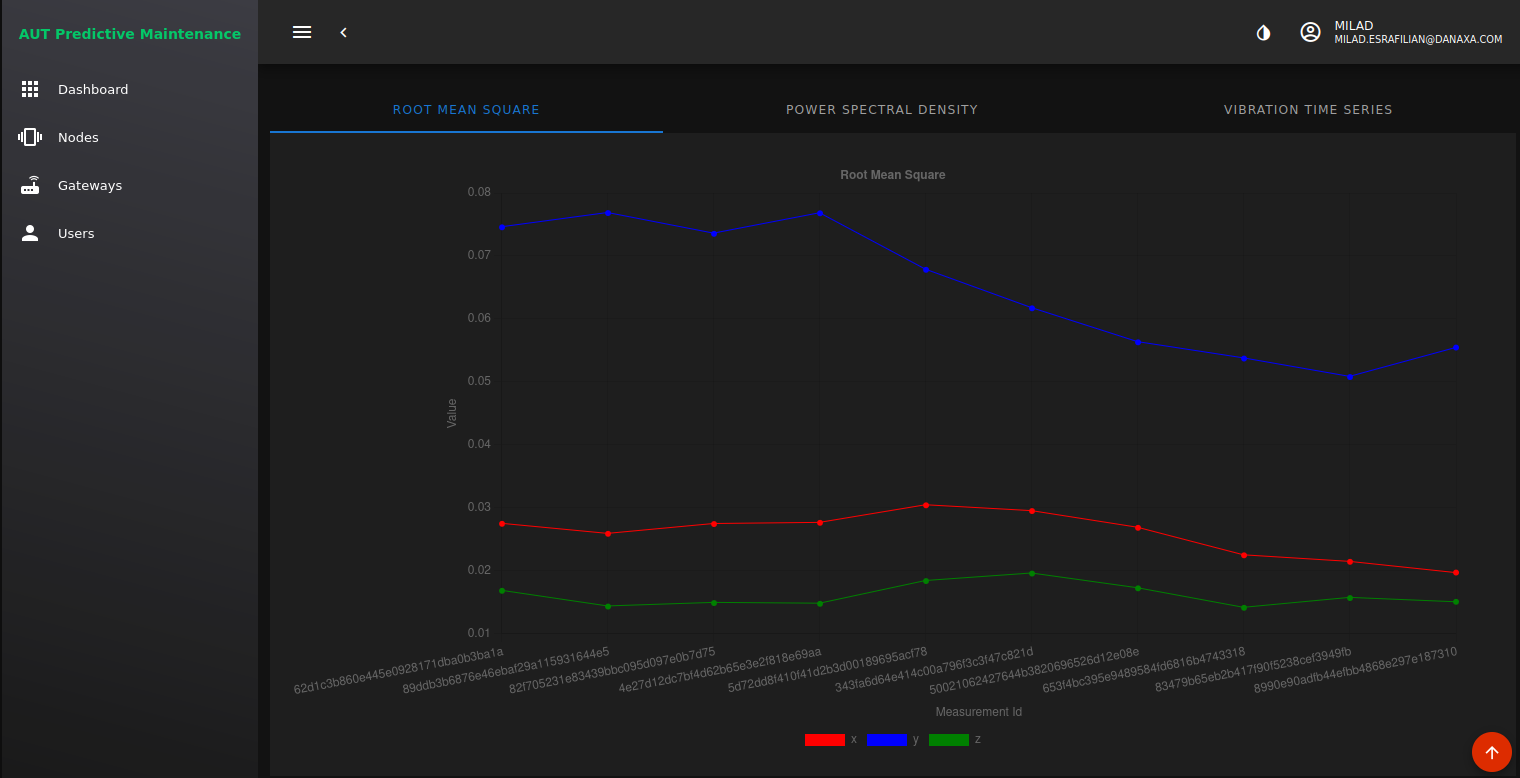
\includegraphics[scale=.38]{rms_chart.png}
\caption{نمودار ریشه میانگین مربع}\label{fig:rms_chart}
\end{figure}

برای نمایش نمودار چگالی طیفی توان، ابتدا شناسه اندازه‌گیری باید از ورودی کشویی انتخاب شود. پس از انتخاب، دو درخواست برای دریافت مقادیر \lr{PSD} و قله‌ها به سرور ارسال می‌شود. سپس قله‌ها مطابق \cref{fig:psd_chart} به همراه نمودار چگالی طیفی توان با نقاط بزرگ‌تر نشان داده می‌شوند.

\begin{figure}[!h]
\centering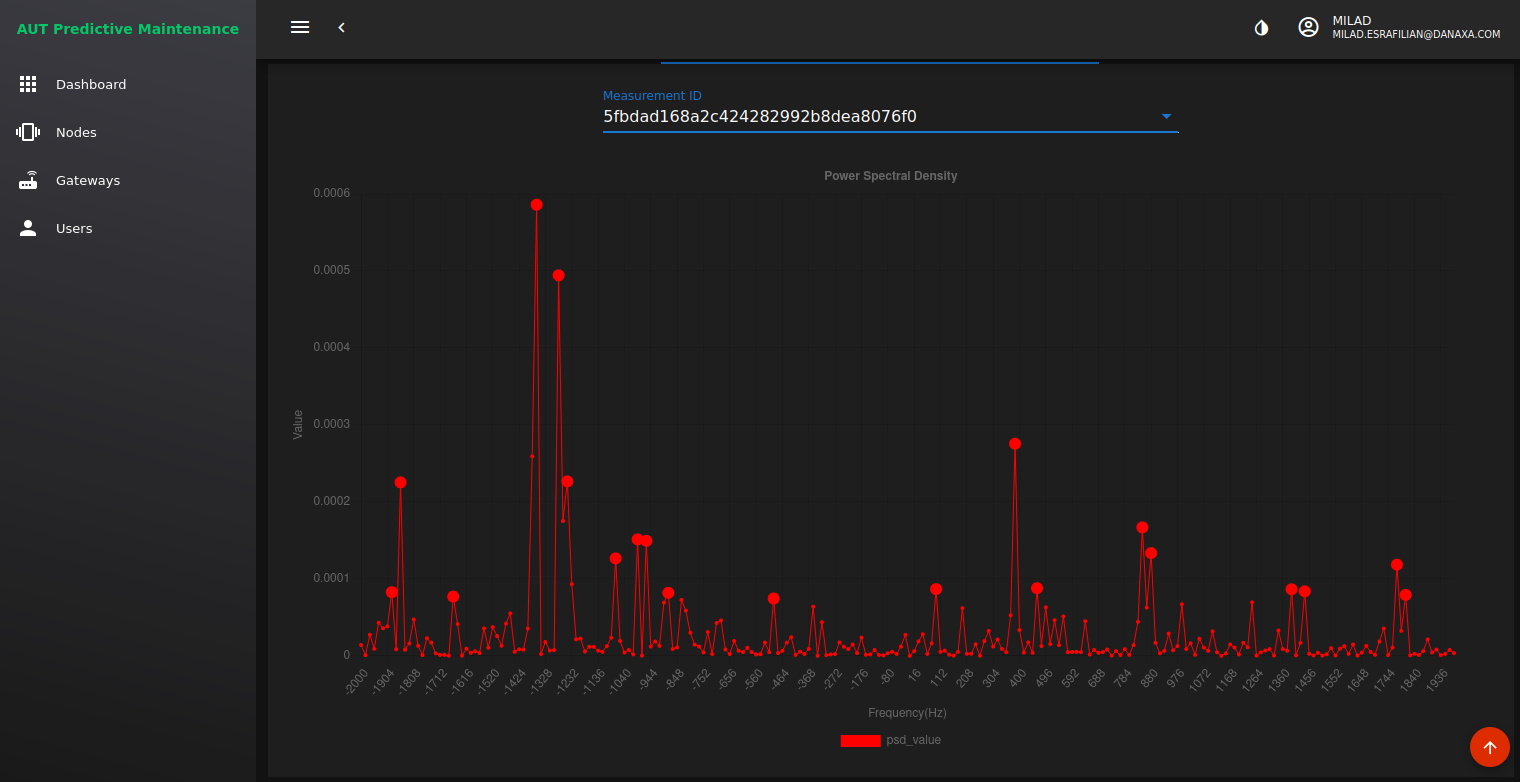
\includegraphics[scale=.38]{psd_chart.png}
\caption{نمودار چگالی طیفی توان}\label{fig:psd_chart}
\end{figure}

سری زمانی ارتعاش، داده‌های خام سه محور را مطابق \cref{fig:vdt_chart} در یک نمودار نشان داده می‌شود. در این برگه نیز لازم است ابتدا شناسه اندازه‌گیری انتخاب شود تا نمودار نمایش داده شود.

\begin{figure}[!h]
\centering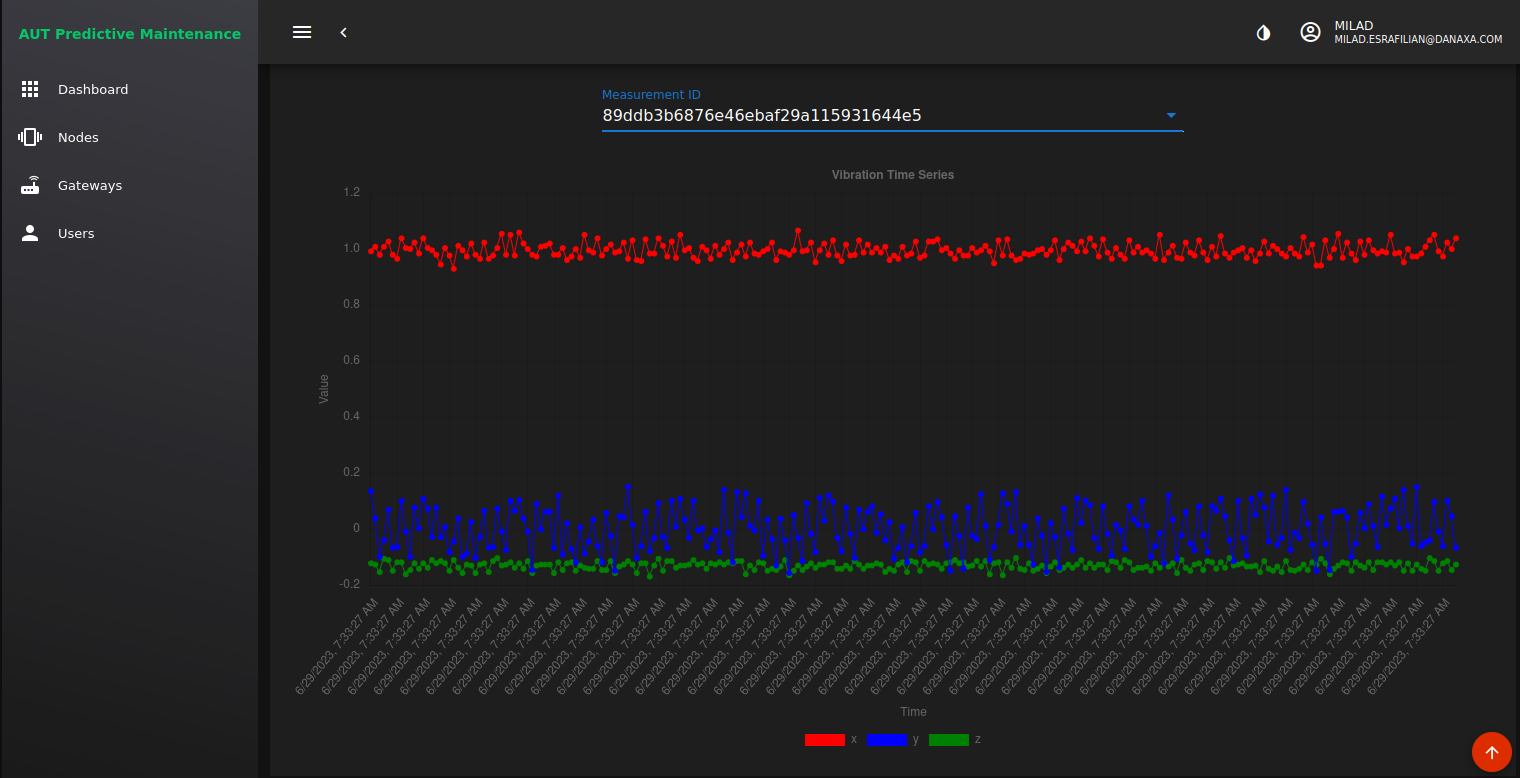
\includegraphics[scale=.38]{vdt_chart.png}
\caption{نمودار سری زمانی ارتعاش}\label{fig:vdt_chart}
\end{figure}

\section{نتیجه‌گیری و جمع‌بندی}

در این بخش در مورد نحوه پیاده‌سازی سیستم صحبت کردیم. ابتدا در مورد ساختار کلی سیستم صحبت کردیم، سپس در مورد نحوه پیاده سازی کد در آردوینو برای گره‌ها صحبت کردیم. سپس دروازه و تمام فایل‌های آن را توضیح دادیم. سپس در مورد پیش‌پردازش و هنجارسازی داده‌ها صحبت کردیم. پس از آن در مورد طرز کار و کتابخانه پایگاه داده سری زمانی برای نوشتن و چستجوی داده‌ها صحبت کردیم و در پایان در مورد برنامه وب و نحوه کار با آن صحبت کردیم و چند تصویر از خروجی را نیز نشان دادیم.
